\chapter{Sequence Tagging}

\section{Part of Speech (PoS) Tagging}

\dfn{PoS Tagging}{

}

\qs{}{Perché studiare PoS?}

\begin{itemize}
  \item Text-to-Speech: la pronuncia di alcune parole cambia in base alla loro parte nel discorso. 
  \item Scrivere regexps: per cercare le frasi principali. 
  \item Input per un parser completo. 
  \item MT (Machine Translation): riordinare aggettivi e nomi nelle traduzioni. 
  \item Si potrebbe volere distinguere tra aggettivi o altre parti del discorso. 
  \item Si potrebbe voler studiare cambiamenti linguistici come la ceazione di nuove parole o shifting del significato.
\end{itemize}

\begin{figure}[h]
    \centering
    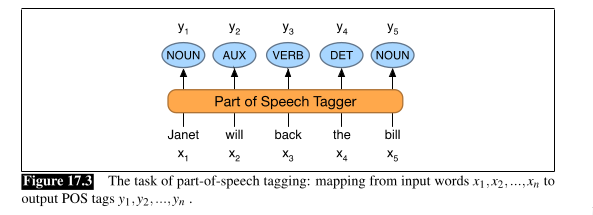
\includegraphics[scale=0.6]{02/PoS}
    \caption{Part of Speech Tagging.}
\end{figure}

\qs{}{Quanto è difficile il PoS Tagging?}

\begin{itemize}
  \item 85\% delle parole non sono ambigue. 
  \item 15\% delle parole sono ambigue e molto frequenti (il 60\% delle parole che si ascoltano sono ambigue).
\end{itemize}

\qs{}{Quanti tag sono corretti?}

\begin{itemize}
  \item Attualmente 97\%. 
  \item Una \textit{baseline} del 92\% è possibile con il metodo più banalie:
    \begin{itemize}
      \item Si dà un tag a ogni parola con il suo significato più frequente. 
      \item Si dà un tag nome alle parole sconosciute.
    \end{itemize}
\end{itemize}

\begin{figure}[h]
    \centering
    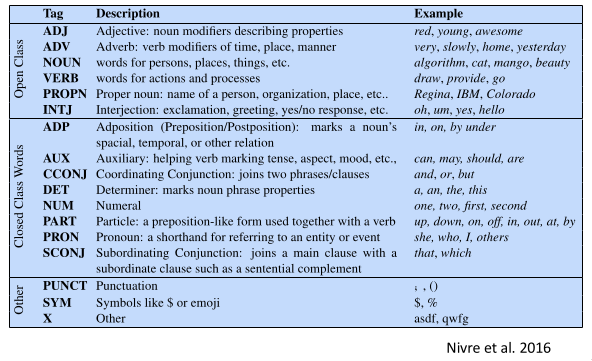
\includegraphics[scale=0.7]{02/tagset}
    \caption{Tagset.}
\end{figure}


